\documentclass[lecture.tex]{subfiles}

\begin{document}

\exercice{}
%\video{https://youtu.be/blablabla}
\enonce{rdm-0060}{Flexion}

Une poutre de longueur $3L$ est bi-appuyée en $A$ et $B$ (rotule en $A$ et appui ponctuel en $B$) et soumise à un effort ponctuel $F$ à son extrémité droite en $C$, tel que présenté sur le schéma ci-dessous.

\begin{figure}[h!]
  \centering
  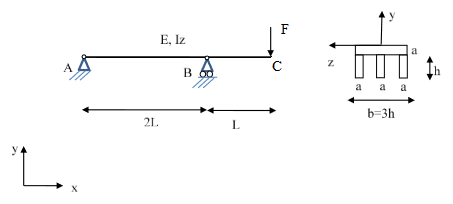
\includegraphics[scale=1.1]{fig1-rdm-0060.png}
\end{figure}

\medskip

\textbf{Données :}

\begin{itemize}[label =\ding{110}, font =\tiny ]
  \item Effort ponctuel : $F$
  \item Module d'Young : $E$
  \item Longueur : $3L$
  \item Hauteur de la section : $h$
  \item Largeur de la section : $b$
  \item Largeur des sous-sections rectangulaires : $a$
  \item Moment d'inertie : $I_z$
\end{itemize}

\bigskip

\begin{enumerate}
  \item Déterminer le degré d'hyperstaticité du système.
  \item A l'aide d'une étude statique, déterminer les efforts de liaisons.
  \item Déterminer les efforts internes dans la poutre et tracer les diagrammes associés.
  \item Déterminer la position du centre de géométrie puis le moment d'inertie $I_z$ de la section de poutre. On étudiera la section en la décomposant en quatre sous sections comme illustré sur le schéma (trois sous-sections rectangulaires verticales de côté a et h et une horizontale de côté $a$ et $b=3 h)$.
  \item %
  \begin{enumerate}
    \item Déterminez l'expression de la contrainte normale pour chacun des tronçons, en fonction de l'abscisse $x$.
    \item Pour chacun des tronçons, sur le schéma d'une section, tracez l'allure de l'évolution de la contrainte normale et précisez les zones où les points subissent de la traction ou de la compression.
    \item Précisez le lieu (abscisse et position dans la section) où la contrainte normale est maximale, puis la calculer.
  \end{enumerate}
  \item Ecrire les conditions aux limites du système.
  \item Déterminer l'expression de la flèche et de la rotation le long de la poutre.
  \item En déduire la flèche et la rotation maximales.
\end{enumerate}

\finenonce{rdm-0060}
\finexercice


\end{document}
